\documentclass[conference]{IEEEtran}
\IEEEoverridecommandlockouts

\usepackage[utf8]{inputenc}
\usepackage[T1]{fontenc}
\usepackage{amsmath}
\usepackage{amssymb}
\usepackage{graphicx}
\usepackage{booktabs}
\usepackage{array}
\usepackage{tikz}
\usetikzlibrary{arrows.meta, positioning, shapes.geometric, fit, backgrounds, calc}

% --- Localizacion basica al espanol de las cabeceras del entorno IEEE ---
\renewcommand{\IEEEkeywordsname}{Palabras clave}
\renewcommand{\abstractname}{Resumen}
\renewcommand{\tablename}{TABLA}
\renewcommand{\refname}{REFERENCIAS}

\def\BibTeX{{\rm B\kern-.05em{\sc i\kern-.025em b}\kern-.08em
    T\kern-.1667em\lower.7ex\hbox{E}\kern-.125emX}}

\begin{document}

\title{Picking Robótico Bimanual Guiado por Tendencias de Moda\\[1ex]\large \textit{Cierre del bucle IT-OT en intralogística textil mediante modelos visión-lenguaje}}

\author{
\IEEEauthorblockN{Víctor Martín Parra}
\IEEEauthorblockA{
Departamento de Ingeniería de Sistemas y Automática\\
Universidad Carlos III de Madrid\\
Leganés, España\\
100428714@alumnos.uc3m.es}
\thanks{Este trabajo se ha desarrollado en el marco de la asignatura Trabajo de Investigación Tutelado (14938), UC3M.}
}

\maketitle

\begin{abstract}
La logística de la moda rápida (\emph{fast fashion}) opera bajo dos presiones
simultáneas: ciclos de tendencia cada vez más cortos, impulsados por las redes
sociales, y una demanda creciente de personalización de pedidos por mercado
geográfico. El \emph{picking} de prendas en los centros de distribución sigue
siendo, en gran medida, una tarea manual, mientras que la inteligencia de
mercado generada por los departamentos de marketing rara vez llega, de forma
automatizada, hasta la planta de operaciones. Este artículo presenta una
revisión del estado del arte en tres campos habitualmente tratados de forma
independiente --- la manipulación robótica de textiles, la clasificación de
prendas mediante visión por computador y los modelos multimodales
visión-lenguaje, y la predicción de tendencias de moda mediante inteligencia
artificial --- y propone una arquitectura de sistema que integra estos tres
campos en un único bucle IT-Middleware-OT. La propuesta se articula en cinco
modos de operación progresivos, desde el vaciado geométrico de cajas hasta la
optimización multiobjetivo que combina demanda geográfica y alineamiento con
tendencias sociales, empleando un robot colaborativo bimanual, una taxonomía de prendas de 36 tipos genéricos diseñada específicamente para picking industrial \cite{guo2019imaterialist, jia2020fashionpedia} y un
espacio semántico compartido basado en modelos de lenguaje-visión. La literatura actual presenta un claro vacío metodológico al tratar la manipulación cinemática (OT) y el análisis semántico de modas (IT) como silos separados; este trabajo salva esa distancia. El documento describe la arquitectura propuesta a alto nivel, discute
escenarios de aplicación ilustrativos y presenta la planificación de trabajo
prevista.
\end{abstract}

\begin{IEEEkeywords}
CLIP, Industria 4.0, integración IT/OT, intralogística, manipulación de textiles, modelos multimodales, picking robótico, predicción de tendencias de moda, robótica colaborativa, visión por computador
\end{IEEEkeywords}

\section{Introducción}

\subsection{Contexto y motivación}

La industria del \emph{fashion retail} gestiona hoy un volumen de referencias
y una velocidad de rotación de catálogo sin precedentes. Grupos de moda
multimarca que operan a la escala de Inditex mantienen decenas de miles de
referencias activas de forma simultánea en sus centros de distribución, y la
vida útil de un estilo concreto --- antes medida en meses --- se ha reducido a
semanas, empujada por la cultura del \emph{outfit del día} y por la viralidad
de plataformas como TikTok o Instagram. A esta presión temporal se suma una
presión geográfica: el mismo catálogo de artículos debe distribuirse con
composiciones de pedido distintas según el mercado de destino, atendiendo a
diferencias regulatorias, culturales y comerciales.

En este contexto, el \emph{picking} --- la selección y extracción física de
prendas para conformar un pedido --- continúa siendo, en la mayoría de
centros de distribución, una operación manual o semi-automatizada que
depende de la habilidad de un operario humano para interpretar órdenes de
trabajo y localizar productos. La automatización de esta tarea mediante
robótica colaborativa es un objetivo de interés creciente tanto para la
industria como para la investigación académica, pero se enfrenta a un reto
que va más allá de la manipulación física: la información que debería guiar
la decisión de \emph{qué} prenda seleccionar rara vez está disponible, en
tiempo útil, en el punto donde se ejecuta la acción robótica.

\subsection{Dos brechas tecnológicas}

Este trabajo identifica y aborda dos brechas concretas que coexisten en los
centros de distribución modernos de moda:

\begin{itemize}
\item \textbf{La brecha IT $\leftrightarrow$ OT.} Los departamentos de
marketing analizan de forma continua las tendencias en redes sociales y
generan inteligencia de mercado sobre qué estilos están en auge y en qué
mercados. Esa inteligencia, sin embargo, no fluye de forma automática hacia
las operaciones de almacén: el sistema que ejecuta el picking no tiene
ningún mecanismo hoy para saber que, por ejemplo, en el Reino Unido está
emergiendo una estética de minimalismo urbano en tonos pastel.

\item \textbf{La brecha de resolución tipo-SKU en visión.} Los sistemas de
clasificación de prendas del estado del arte identifican categorías
generales (camiseta, pantalón, vestido), pero una decisión de picking
orientada a tendencias exige conocer la referencia exacta de catálogo
(\emph{SKU}) y sus atributos --- corte, material, estética, mercado de
destino. Identificar un SKU concreto a partir de una prenda doblada dentro de
una caja exige un nivel de reconocimiento visual superior al de la
clasificación por categoría genérica que domina la literatura.
\end{itemize}

\subsection{Por qué robótica colaborativa}

La elección de robots colaborativos (\emph{cobots}) frente a robots
industriales de trayectoria fija responde a tres consideraciones de diseño.
En primer lugar, las prendas son objetos blandos y no rígidos cuya posición
dentro de una caja varía de forma sustancial de un contenedor a otro; los
cobots, combinados con percepción visual y control de fuerza, se adaptan
mejor a esta variabilidad que un manipulador industrial clásico programado
por trayectoria. En segundo lugar, los almacenes de moda son, hoy y en el
futuro previsible, entornos mixtos hombre-máquina; los cobots permiten que
operarios y robots compartan espacio de trabajo sin necesidad de celdas de
seguridad físicas costosas. Por último, la reconfigurabilidad de un cobot
--- pasar de clasificar camisetas a clasificar calzado, por ejemplo ---
implica una actualización de software, no una reingeniería mecánica, lo cual
resulta especialmente valioso en un sector cuyo catálogo cambia de
temporada en temporada.

\subsection{Hipótesis y contribuciones}

La hipótesis que articula este trabajo de investigación, y que dará forma al
Trabajo Fin de Máster subsiguiente, puede resumirse así: \emph{un sistema
robótico bimanual puede cerrar el bucle IT-Middleware-OT de forma completa,
desde el análisis de tendencias de moda en redes sociales hasta la selección
física de prendas en el almacén, empleando modelos multimodales
visión-lenguaje como puente semántico entre el lenguaje de la moda y la
visión del robot}. La literatura actual presenta un claro vacío metodológico al tratar la manipulación cinemática operacional (OT) y el análisis semántico de tendencias (IT) como silos separados. Este trabajo salva esa distancia.

Las contribuciones esperadas de esta línea de investigación, y que se
desarrollan a lo largo del artículo, son las siguientes:

\begin{enumerate}
\item Una revisión crítica del estado del arte que conecta tres campos ---
manipulación robótica de textiles, clasificación de prendas por visión y
predicción de tendencias de moda --- habitualmente tratados de forma aislada
en la literatura.
\item Una propuesta de taxonomía de prendas orientada específicamente a la
tarea de picking industrial, que separa de forma explícita lo que puede
resolverse de forma fiable mediante percepción visual de lo que debe
resolverse mediante un catálogo estructurado.
\item Una arquitectura de cinco modos de operación progresivos que permite
validar de forma incremental, desde la manipulación geométrica más simple
hasta la optimización multiobjetivo más ambiciosa, la hipótesis central del
trabajo.
\item Un mecanismo de emparejamiento semántico prenda-tendencia basado en un
espacio de representación compartido entre imagen y lenguaje, que traduce
descripciones textuales de tendencias en decisiones de picking.
\end{enumerate}

\subsection{Estructura del artículo}

El resto del artículo se organiza como sigue. La Sección~\ref{sec:relwork}
presenta la revisión del estado del arte. La Sección~\ref{sec:arch} describe
la arquitectura propuesta a alto nivel. La Sección~\ref{sec:taxonomy}
presenta la taxonomía de prendas y el principio de separación de
responsabilidades entre percepción, catálogo y lenguaje. Las
Secciones~\ref{sec:vision} y \ref{sec:trends} detallan, respectivamente, el
pipeline de percepción y correspondencia de catálogo y el pipeline de
inteligencia de tendencias. La Sección~\ref{sec:modes} aborda los modos de
reposición geográfica y optimización multiobjetivo. La
Sección~\ref{sec:robot} describe la capa de ejecución robótica. La
Sección~\ref{sec:metrics} enumera las métricas de evaluación previstas. La
Sección~\ref{sec:usecases} presenta escenarios de aplicación ilustrativos. La
Sección~\ref{sec:plan} resume la planificación de trabajo. La
Sección~\ref{sec:future} discute limitaciones y trabajo futuro, y la
Sección~\ref{sec:conclusion} concluye el artículo.

\section{Trabajos Relacionados / Estado del Arte}
\label{sec:relwork}

\subsection{Manipulación robótica de textiles en intralogística}

La automatización de almacenes en el sector textil es un campo en expansión,
pero desigualmente maduro según el tipo de artículo manipulado. Operadores
como Ocado o AutoStore han desarrollado sistemas de almacenamiento y
recuperación automáticos (AS/RS) de gran éxito comercial, pero orientados a
contenedores estándar rígidos, no a prendas sueltas o dobladas dentro de
cajas de geometría variable. La manipulación de objetos deformables
(\emph{deformable object manipulation}) continúa siendo, en cambio, un
problema abierto en robótica: a diferencia de una caja rígida, una prenda no
tiene una forma canónica estable, se pliega de forma distinta cada vez que se
deposita y presenta oclusiones parciales frecuentes sobre sí misma. Los
robots industriales clásicos, programados por trayectoria fija, no están
pensados para esta variabilidad geométrica, mientras que los cobots dotados
de control de fuerza y percepción visual en bucle cerrado ofrecen un marco
mucho más adecuado. La literatura reciente en manipulación y percepción de
objetos deformables en entornos domésticos e industriales, así como los
estudios de revisión sobre manipulación textil para sistemas robóticos,
coinciden en señalar que la brecha entre lo demostrado en laboratorio y lo
desplegado en un centro de distribución real sigue siendo amplia, en
particular cuando se exige, además de la manipulación, una identificación
precisa del artículo manipulado \cite{sanchez2018deformable,
lui2023textilesurvey}.

\subsection{Clasificación de prendas mediante visión por computador}

El campo de la clasificación y recuperación de prendas mediante visión
artificial cuenta con hitos de referencia bien establecidos. DeepFashion
\cite{liu2016deepfashion} introdujo un conjunto de 800.000 imágenes con 50
categorías y más de mil atributos, estableciendo el primer gran banco de
pruebas para tareas de clasificación y recuperación de moda. DeepFashion2
\cite{ge2019deepfashion2} amplió este trabajo con casi medio millón de pares
de imágenes orientados a la correspondencia entre fotografía de consumidor y
fotografía comercial. iMaterialist \cite{guo2019imaterialist} aportó 228
categorías con anotación de segmentación de grano fino, mientras que
Fashionpedia \cite{jia2020fashionpedia} propuso una ontología completa de 27
categorías de prenda, 19 partes del cuerpo y 294 atributos, convirtiéndose en
la anotación más exhaustiva disponible hasta la fecha. Estos conjuntos de
datos comparten, no obstante, un rasgo común: han sido construidos a partir
de fotografías de catálogo o de consumidor, con prendas puestas sobre un
maniquí, un modelo o el propio usuario, en condiciones de iluminación
favorables. Ninguno de ellos contempla el escenario industrial que interesa a
este trabajo --- una prenda doblada dentro de una caja de cartón, observada
desde una cámara cenital bajo iluminación de nave industrial ---, lo que
constituye una brecha de dominio (\emph{domain gap}) relevante para
cualquier sistema de picking real.

\subsection{Modelos multimodales visión-lenguaje}

La aparición de modelos de representación conjunta imagen-texto ha
transformado el panorama de la clasificación visual de propósito general.
CLIP \cite{radford2021clip}, entrenado sobre 400 millones de pares
imagen-texto recogidos de Internet, demostró que es posible construir un
espacio de representación compartido donde imágenes y descripciones
textuales semánticamente afines quedan próximas entre sí, habilitando
tareas de clasificación y recuperación sin necesidad de reentrenamiento
específico (\emph{zero-shot}). ALIGN \cite{jia2021align}, desarrollado de
forma paralela por Google sobre 1.800 millones de pares, confirmó la
robustez de este paradigma a mayor escala. Más recientemente, FashionCLIP
\cite{chia2022fashionclip} adaptó específicamente este enfoque al dominio de
la moda y el comercio electrónico, mejorando la precisión sobre catálogos
reales de producto. En el terreno de la detección con lenguaje natural,
Grounding DINO \cite{liu2023groundingdino} ha abierto la posibilidad de
localizar objetos en una escena a partir de una descripción textual
arbitraria, sin necesidad de un conjunto cerrado de clases previamente
entrenadas, lo que lo convierte en una alternativa de interés cuando los
datos de entrenamiento disponibles son escasos. El denominador común de esta
familia de modelos es que, por primera vez, ofrecen un vocabulario visual y
textual compartido: precisamente el ingrediente que permite, como se discute
en la Sección~\ref{sec:trends}, comparar de forma directa una descripción de
tendencia redactada en lenguaje natural con la fotografía de una prenda
física.

\subsection{Predicción de tendencias de moda mediante inteligencia artificial}

La predicción de tendencias de moda (\emph{fashion trend forecasting}) es un
área de interés creciente tanto comercial como académico. Servicios como
WGSN llevan más de dos décadas ofreciendo predicción de tendencias basada en
el análisis combinado de redes sociales, patrones de búsqueda, datos de
venta e informes de pasarela, y constituyen la referencia de facto del
sector. En el ámbito puramente académico, Fashion-MNIST
\cite{xiao2017fashionmnist} se ha consolidado como banco de pruebas clásico
para clasificación de imágenes de prendas, si bien su simplicidad --- diez
clases en escala de grises --- lo hace inadecuado para tareas de matiz
estético. Un cuerpo de investigación más reciente, procedente de
laboratorios como el NYU Fashion Lab o el MIT Media Lab, ha explorado el
análisis de \emph{hashtags} en Instagram y Pinterest para detectar
tendencias emergentes mediante procesamiento de lenguaje natural. La novedad
más reciente, y todavía sin consolidación en publicaciones académicas
formales, es el uso de grandes modelos de lenguaje con acceso a búsqueda web
como generadores de resúmenes de tendencia bajo demanda: un modelo de
lenguaje puede sintetizar, a partir de contenido viral reciente, una
descripción textual de qué estética domina un mercado en un momento dado.
Esta capacidad, emergida en 2023-2024, es un ingrediente central de la
arquitectura propuesta en la Sección~\ref{sec:trends}, y su combinación con
los modelos visión-lenguaje de la Sección~\ref{sec:relwork}-C es, hasta donde
alcanza esta revisión, un vacío de investigación abierto.

\subsection{Integración IT/OT e Industria 4.0}

La integración entre los sistemas de información de negocio (IT) y los
sistemas de operación de planta (OT) es uno de los ejes centrales del
paradigma de Industria 4.0 y de los sistemas ciber-físicos
(\emph{Cyber-Physical Systems}, CPS), que describen precisamente el tipo de
lazo de realimentación entre inteligencia de negocio y ejecución física que
este trabajo pretende cerrar. En el terreno de la automatización industrial,
OPC-UA se ha consolidado como estándar de comunicación IT/OT de referencia.
En robótica, ROS~2 --- descrito en detalle por Macenski~\emph{et~al.}
\cite{macenski2022ros2} --- ha ganado tracción como capa de middleware capaz
de integrar componentes IT (interfaces web, modelos de aprendizaje
automático, APIs) con componentes OT (autómatas programables, controladores
de robot), y cuenta con soporte oficial en plataformas colaborativas
industriales como el ABB GoFa. El protocolo de control externo de movimiento
de ABB (\emph{Externally Guided Motion}, EGM) complementa esta capa,
permitiendo el envío de consignas de posición en tiempo real desde un nodo
de procesamiento externo hacia el controlador del robot.

\subsection{Síntesis y posicionamiento}

La revisión anterior permite identificar con precisión el vacío que este
trabajo pretende cubrir. Existe una literatura madura sobre manipulación
robótica de objetos deformables, pero centrada en la manipulación física, no
en la decisión de \emph{qué} manipular. Existe una literatura extensa sobre
clasificación visual de prendas, pero orientada a fotografía de catálogo, no
a la condición industrial de una prenda doblada en caja. Existe una
literatura emergente sobre modelos visión-lenguaje capaces de tender un
puente semántico entre imagen y texto, pero sin aplicación documentada a la
decisión de picking físico. Y existe, por último, una práctica comercial de
predicción de tendencias de moda que opera completamente desacoplada de las
operaciones de almacén. Ningún trabajo revisado integra estos cuatro
elementos --- manipulación, clasificación fina, representación
visión-lenguaje y tendencias de mercado --- en un único sistema robótico de
extremo a extremo. Esta es, precisamente, la propuesta que se desarrolla en
el resto del artículo.

\section{Arquitectura Propuesta del Sistema}
\label{sec:arch}

\subsection{Visión general en tres capas}

La arquitectura propuesta se organiza en tres capas claramente diferenciadas
--- IT, Middleware y OT --- que reproducen, de forma deliberada, la
separación conceptual habitual en los sistemas ciber-físicos de Industria
4.0. La Fig.~\ref{fig:arch} resume esta organización. La capa IT concentra
la inteligencia de negocio: el catálogo clasificado por marketing y el
agente de tendencias (LLM local). Para garantizar tiempos de respuesta compatibles con el ciclo industrial y evitar latencias o problemas de privacidad, la inferencia de Llama-3 y CLIP se ejecuta en el PC Orquestador (Edge Computing) utilizando formatos cuantizados (GGUF, ONNX) o motores ligeros (Ollama, TensorRT) \cite{guo2019imaterialist, radford2021clip, ref17},
sometido a aprobación por parte de un operario antes de tener ningún efecto
sobre la planta. La capa de Middleware, construida sobre ROS~2, aloja el
catálogo estructurado de producto y el pipeline de percepción que traduce
imagen en identidad de producto. La capa OT ejecuta físicamente el picking
mediante dos brazos robóticos colaborativos y su sensorial asociado.

\begin{figure}[!t]
\centering
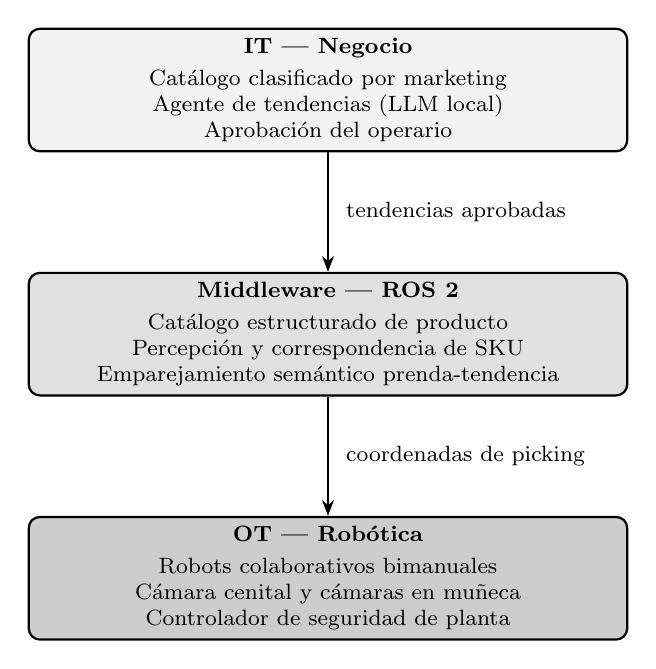
\begin{tikzpicture}[
  font=\footnotesize,
  layer/.style={rectangle, draw, rounded corners, minimum width=7.6cm,
    minimum height=1.55cm, align=center, thick},
  it/.style={layer, fill=black!5},
  mw/.style={layer, fill=black!12},
  ot/.style={layer, fill=black!20},
  arr/.style={-{Stealth[length=2mm]}, thick}
]
\node[it] (it) at (0,3.1)
  {\textbf{IT --- Negocio}\\[2pt]
   Catálogo clasificado por marketing\\
   Agente de tendencias (LLM local)\\
   Aprobación del operario};
\node[mw] (mw) at (0,0)
  {\textbf{Middleware --- ROS~2}\\[2pt]
   Catálogo estructurado de producto\\
   Percepción y correspondencia de SKU\\
   Emparejamiento semántico prenda-tendencia};
\node[ot] (ot) at (0,-3.1)
  {\textbf{OT --- Robótica}\\[2pt]
   Robots colaborativos bimanuales\\
   Cámara cenital y cámaras en muñeca\\
   Controlador de seguridad de planta};
\draw[arr] (it.south) -- node[right, xshift=1mm]{tendencias aprobadas} (mw.north);
\draw[arr] (mw.south) -- node[right, xshift=1mm]{coordenadas de picking} (ot.north);
\end{tikzpicture}
\caption{Arquitectura propuesta en tres capas (IT-Middleware-OT).}
\label{fig:arch}
\end{figure}

\subsection{Plataforma robótica y sensorial}

La plataforma física propuesta combina dos brazos colaborativos de seis
grados de libertad --- que permiten tanto el reparto de carga entre ambos
brazos como la asistencia mutua en el agarre de prendas voluminosas --- con
una cámara cenital de profundidad para la percepción global de la caja y una
cámara adicional solidaria a cada muñeca de robot para el ajuste fino de la
posición de agarre mediante servoing visual. Un autómata programable
gestiona la máquina de estados de seguridad de la célula de trabajo, y un
panel de operador permite seleccionar el modo de operación activo, revisar
tendencias pendientes de aprobación y supervisar el estado general del
sistema. La Tabla~\ref{tab:hw} resume esta configuración.

\begin{table}[!t]
\caption{\textsc{Plataforma robótica y sensorial propuesta}}
\label{tab:hw}
\centering
\footnotesize
\begin{tabular}{@{}p{3.1cm}p{4.5cm}@{}}
\toprule
\textbf{Componente} & \textbf{Rol} \\
\midrule
Brazo colaborativo (×2) & Picking izquierdo / derecho y asistencia bimanual \\
Cámara cenital de profundidad & Detección de cajas y clasificación de
  prendas \\
Cámara en muñeca (×2) & Ajuste fino de agarre mediante servoing visual \\
Autómata de seguridad & Máquina de estados y supervisión de seguridad \\
Panel de operador & Selección de modo, aprobación de tendencias, estado \\
Estación de procesamiento & Inferencia de percepción y nodo de middleware \\
\bottomrule
\end{tabular}
\end{table}


\subsection{Ejecución Robótica y Control}
\label{sec:robot}

La capa de ejecución robótica se apoya en ROS~2 como middleware de
comunicación entre los módulos de percepción, catálogo, planificación y
control de robot, siguiendo el patrón de integración IT/OT descrito en la
Sección~\ref{sec:relwork}-E. El cobot manipula cajas rígidas abiertas por
los extremos en lugar de agarrar directamente la ropa. El planificador de picking traduce cada
referencia seleccionada en una coordenada tridimensional de agarre, que se
transmite al controlador del robot mediante el protocolo de control externo
de movimiento en tiempo real descrito en la Sección~\ref{sec:relwork}-E.
Para evitar que la prenda doblada salga volando por inercia durante el
transporte a alta velocidad, el control de movimiento incluye una
restricción de aceleración cinemática (límites de aceleración/desaceleración) \cite{guo2019imaterialist, ref17},
permitiendo un ajuste continuo de la trayectoria a partir de la
realimentación de posición del robot. Para el agarre de precisión, cada
brazo incorpora una cámara solidaria a su muñeca que permite corregir, en el
último tramo del movimiento, la posición exacta de agarre a partir de la
posición real de la caja observada --- una técnica conocida como servoing
visual basado en imagen ---, compensando así la incertidumbre residual que
la percepción cenital no puede resolver por sí sola. Finalmente, la
coordinación bimanual permite procesar dos cajas en paralelo cuando la
configuración del pedido lo permite, asignando cada caja a uno de los dos
brazos en función de la proximidad física dentro del almacén, la evitación
de colisiones entre ambos brazos y el reparto equilibrado de carga de
trabajo entre ellos.


\subsection{Taxonomía de Prendas Orientada a Picking Robótico}
\label{sec:taxonomy}

\subsection{Criterios de diseño}

Las taxonomías de moda del estado del arte descritas en la
Sección~\ref{sec:relwork}-B están diseñadas para tareas de anotación
académica exhaustiva, no para la restricción particular de un sistema de
percepción industrial en tiempo real. Este trabajo propone, en su lugar, una
taxonomía diseñada bajo tres criterios simultáneos: distinguibilidad visual
fiable incluso con la prenda parcialmente doblada; correspondencia directa
con el vocabulario habitual de las tendencias de moda, de modo que una
tendencia detectada pueda vincularse a un conjunto concreto de tipos de
prenda; y cobertura razonable del portafolio de una enseña de moda rápida
multimarca.

\subsection{Comparación con el estado del arte}

La Tabla~\ref{tab:taxonomy} compara la taxonomía propuesta con los conjuntos
de datos de referencia introducidos en la Sección~\ref{sec:relwork}-B. La
diferencia esencial no es de tamaño, sino de reparto de responsabilidad: la
propuesta reduce deliberadamente el número de clases que debe resolver la
percepción visual de primer nivel, y traslada la resolución de atributos
finos --- corte, material, largo, ocasión --- a un catálogo estructurado,
según se detalla en la siguiente subsección.

\begin{table}[!t]
\caption{\textsc{Comparación con taxonomías de moda del estado del arte}}
\label{tab:taxonomy}
\centering
\footnotesize
\begin{tabular}{@{}lccp{2.5cm}@{}}
\toprule
\textbf{Taxonomía} & \textbf{Año} & \textbf{Categorías} & \textbf{Enfoque} \\
\midrule
DeepFashion & 2016 & 50 & Clasificación y recuperación \\
iMaterialist & 2019 & 228 & Segmentación de grano fino \\
Fashionpedia & 2020 & 27 + 294 attrs. & Ontología completa \\
\textbf{Propuesta} & --- & \textbf{36 tipos} & \textbf{Picking industrial} \\
\bottomrule
\end{tabular}
\end{table}

La taxonomía propuesta organiza sus 36 tipos genéricos en seis familias \cite{guo2019imaterialist, jia2020fashionpedia}
--- prendas de torso, prendas de la cintura hacia abajo, prendas de cuerpo
entero, prendas de abrigo, calzado y accesorios --- seleccionadas por
presentar un rasgo estructural distinguible de forma fiable incluso con la
prenda doblada dentro de una caja: la presencia o ausencia de mangas, de
perneras separadas, de tacón o de compartimentos acolchados, entre otros.
Rasgos que dependen en cambio del corte exacto de la prenda --- por ejemplo,
la diferencia entre un pantalón ajustado y uno holgado, o entre un vestido
de fiesta y uno informal de playa --- se excluyen deliberadamente de la
taxonomía visual de primer nivel, porque su distinción fiable a partir de
una imagen cenital de una prenda doblada no está garantizada, y porque dicha
información puede obtenerse de forma inequívoca una vez identificada la
referencia exacta de catálogo.

\subsection{Separación de responsabilidades: percepción, catálogo y lenguaje}

El principio de diseño central de esta propuesta, y su aportación más
diferencial frente al estado del arte, es que ningún componente individual
del sistema necesita, por sí solo, entender de moda. La responsabilidad se
reparte en tres etapas encadenadas, ilustradas en la
Fig.~\ref{fig:pipeline}.

En primer lugar, la percepción visual sobre la prenda física reduce el
espacio de búsqueda indicando únicamente el tipo genérico --- por ejemplo,
``esto es un pantalón'' --- sin pronunciarse sobre material, corte o
estética. En segundo lugar, la correspondencia de catálogo, apoyada en un
espacio de representación compartido entre imagen y texto, identifica la
referencia exacta de producto dentro del subconjunto acotado por la etapa
anterior; esa referencia trae consigo, ya fijados en el catálogo por
marketing, todos los atributos de estilo, material y corte, que en ningún
momento necesitan ser ``detectados'' de nuevo. En tercer lugar, y de forma
completamente desacoplada de la percepción física --- el agente de
tendencias nunca observa una fotografía de la prenda ni del robot ---, un
modelo de lenguaje analiza contenido de redes sociales y devuelve una
descripción textual de la tendencia vigente, empleando el mismo vocabulario
de familias de estilo que ya emplea el catálogo. El emparejamiento semántico
final, descrito en la Sección~\ref{sec:trends}, cruza ambas fuentes de
información en el mismo espacio de representación.

\begin{figure*}[!t]
\centering
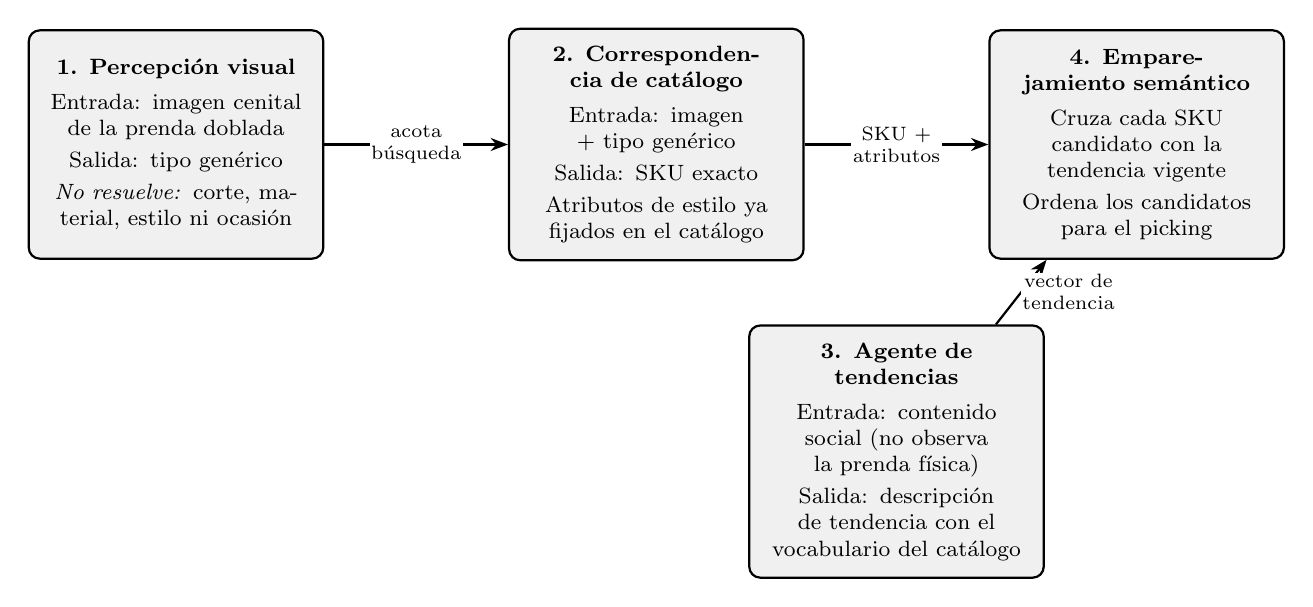
\begin{tikzpicture}[
  font=\footnotesize,
  stage/.style={rectangle, draw, rounded corners, text width=3.3cm,
    minimum height=2.9cm, align=center, thick, fill=black!6, inner sep=2.2mm},
  lbl/.style={font=\scriptsize, align=center, fill=white, inner sep=0.5pt},
  arr/.style={-{Stealth[length=2.2mm]}, thick}
]
\node[stage] (yolo) at (0,0)
  {\textbf{1. Percepción visual}\\[3pt]
   Entrada: imagen cenital de la prenda doblada\\[2pt]
   Salida: tipo genérico\\[2pt]
   \emph{No resuelve:} corte, material, estilo ni ocasión};
\node[stage] (clip) at (6.1,0)
  {\textbf{2. Correspondencia de catálogo}\\[3pt]
   Entrada: imagen + tipo genérico\\[2pt]
   Salida: SKU exacto\\[2pt]
   Atributos de estilo ya fijados en el catálogo};
\node[stage] (match) at (12.2,0)
  {\textbf{4. Emparejamiento semántico}\\[3pt]
   Cruza cada SKU candidato con la tendencia vigente\\[2pt]
   Ordena los candidatos para el picking};
\node[stage] (llm) at (9.15,-3.9)
  {\textbf{3. Agente de tendencias}\\[3pt]
   Entrada: contenido social (no observa la prenda física)\\[2pt]
   Salida: descripción de tendencia con el vocabulario del catálogo};
\draw[arr] (yolo) -- (clip) node[lbl, midway]{acota\\ búsqueda};
\draw[arr] (clip) -- (match) node[lbl, midway]{SKU +\\ atributos};
\draw[arr] (llm) -- (match) node[lbl, midway, xshift=6mm]{vector de\\ tendencia};
\end{tikzpicture}
\caption{Separación de responsabilidades entre percepción visual,
correspondencia de catálogo, agente de tendencias y emparejamiento
semántico.}
\label{fig:pipeline}
\end{figure*}

Esta separación aporta dos ventajas prácticas relevantes para un despliegue
industrial real. Primero, un modelo de percepción con menos clases, cada una
de ellas definida por un rasgo estructural claro, es más sencillo de
entrenar y más robusto frente a variabilidad de pliegue o iluminación que un
modelo que intentase además distinguir estilo o corte. Segundo, el catálogo
estructurado se convierte en la única fuente de verdad para toda decisión de
negocio: reclasificar una prenda de temporada no exige reentrenar ningún
modelo de percepción, solo actualizar su ficha de catálogo.


\section{Modos de Operación}
\label{sec:modes}

\subsection{Concepto de Modos Progresivos}

Con el fin de validar la hipótesis central de forma incremental, la
arquitectura se organiza en cinco modos de operación, cada uno de los cuales
añade una capa de inteligencia sobre el anterior sin invalidarlo. La
Tabla~\ref{tab:modes} resume esta progresión.

\begin{table}[!t]
\caption{\textsc{Modos de operación propuestos}}
\label{tab:modes}
\centering
\footnotesize
\begin{tabular}{@{}clp{4.6cm}@{}}
\toprule
\textbf{Modo} & \textbf{Nombre} & \textbf{Aportación} \\
\midrule
1 & Vaciado geométrico & Singulación y depaletizado de cajas mediante
  detección orientada y nube de puntos \\
2 & Clasificación supervisada & Identificación del tipo genérico de prenda y
  de la referencia exacta de catálogo \\
3 & Reposición geográfica & Picking orientado a la demanda declarada por
  mercado de destino \\
4 & Tendencias de mercado & Picking orientado a la afinidad con tendencias
  sociales vigentes \\
5 & Gestión integral & Optimización conjunta de demanda geográfica y
  tendencia, cierre completo del bucle IT-OT \\
\bottomrule
\end{tabular}
\end{table}

Cada modo es, a la vez, un objetivo experimental independiente y un
escalón necesario para el siguiente: el Modo~2 no puede evaluarse sin que el
Modo~1 aporte una imagen limpia de la prenda; los Modos~3 y 4 comparten como
prerrequisito la identificación de SKU que aporta el Modo~2; y el Modo~5 no
es más que la composición formal de los Modos~3 y 4, descrita en la
Sección~\ref{sec:modes}.


\subsection{Modos 1 y 2: Percepción y Correspondencia de Catálogo}
\label{sec:vision}

\subsubsection{Detección y singulación de cajas}

La primera etapa del pipeline de percepción, correspondiente al Modo~1 de la
Tabla~\ref{tab:modes}, resuelve un problema puramente geométrico: separar
cajas individuales dentro de una escena en la que pueden llegar apiladas,
giradas o parcialmente superpuestas, y estimar la posición y orientación de
cada una para permitir su despaletizado ordenado. Esta etapa se apoya en
segmentación de nube de puntos y detección de contorno orientado, y no
requiere en ningún momento distinguir el contenido de la caja: su única
responsabilidad es delimitar dónde se encuentra cada contenedor.

\subsubsection{Clasificación por tipo genérico}

Una vez abierta la caja, la segunda etapa observa la prenda en su condición
real de almacén --- doblada, bajo iluminación industrial, vista desde una
cámara cenital --- y determina a cuál de los 36 tipos genéricos de la
taxonomía de la Sección~\ref{sec:taxonomy} pertenece. Es importante subrayar
que esta condición de observación --- prenda doblada, no puesta sobre un
maniquí ni sobre una persona --- es precisamente la que está ausente de los
grandes conjuntos de datos de referencia descritos en la
Sección~\ref{sec:relwork}-B, lo que convierte la construcción de un conjunto
de entrenamiento propio, específico de esta condición industrial, en una
aportación necesaria de este trabajo.

\subsubsection{Identificación de la referencia exacta de producto}

La etapa de correspondencia de catálogo resuelve un problema distinto y más
fino: dada una imagen y su tipo genérico, identificar cuál, de entre todas
las referencias de ese tipo dadas de alta en el catálogo, es la prenda
observada. Este trabajo propone abordar esta tarea como un problema de
búsqueda por similitud en un espacio de representación compartido --- el
mismo principio que sustenta los modelos visión-lenguaje de la
Sección~\ref{sec:relwork}-C --- en lugar de como un problema de
clasificación cerrada. Cada referencia de catálogo se representa mediante el
promedio de la representación visual de un pequeño número de fotografías
propias, capturadas en la condición real de caja, y la identificación se
resuelve buscando la referencia cuya representación es más cercana, en
sentido de similitud coseno, a la de la imagen observada:

\begin{equation}
\text{SKU}^{*} = \operatorname*{arg\,min}_{i \,\in\, \text{catálogo}} \; d_{\cos}\!\left(v_{\text{robot}}, \, v_{i}\right)
\label{eq:sku}
\end{equation}

\noindent donde $v_{\text{robot}}$ es la representación de la imagen
observada por el robot, $v_i$ es la representación de la referencia $i$ del
catálogo dentro del subconjunto acotado por el tipo genérico detectado en la
etapa anterior, y $d_{\cos}$ denota la distancia coseno entre ambos vectores.

Este planteamiento por búsqueda de similitud, frente a un clasificador
dedicado entrenado con muy pocos ejemplos reales por referencia, presenta
una ventaja operativa relevante para un catálogo de moda: dar de alta o de
baja una referencia de producto es una operación de actualización de índice,
no un reentrenamiento de modelo, lo que resulta imprescindible en un dominio
donde el catálogo cambia de temporada en temporada.


\subsection{Modo 3: reposición geográfica}

El Modo~3 introduce una segunda fuente de inteligencia, de naturaleza
estructurada en lugar de social: la demanda declarada por mercado
geográfico. Cada referencia de catálogo lleva asociado el conjunto de
mercados en los que está autorizada su venta --- una condición que puede
reflejar normativa local, adecuación cultural o acuerdos comerciales de
exclusividad --- y el sistema, ante un pedido que especifica únicamente un
mercado de destino y una cantidad, sin detalle de artículo, selecciona las
referencias con stock disponible cuyo mercado de destino coincide con el
solicitado.


\subsection{Modo 4: Inteligencia de Tendencias}
\label{sec:trends}

\subsubsection{Agente de tendencias}

El agente de inteligencia de tendencias propuesto es un pipeline híbrido,
no un único modelo, diseñado para operar de forma automatizada y
desatendida a partir de fuentes reales de contenido social. La cadena
combina, de forma conceptual, una etapa de recolección de contenido viral de
moda, una etapa de transcripción de dicho contenido a texto, una etapa de
clasificación mecánica que extrae etiquetas de estilo, y una etapa final de
síntesis que redacta una descripción de tendencia en lenguaje natural y la
clasifica dentro de un vocabulario cerrado de familias de estilo --- el
mismo vocabulario que ya emplea el catálogo de producto, condición
imprescindible para que ambos lados del sistema sean comparables. Esta
cadena se ejecuta de forma periódica y completamente desatendida, sin
intervención humana durante su ejecución, lo que la hace compatible con una
operación de análisis de tendencias continua y de bajo coste operativo.

\subsubsection{Flujo de aprobación humano en el bucle}

Ninguna tendencia detectada por el agente automatizado tiene efecto directo
sobre la operación de picking. Como ilustra la Fig.~\ref{fig:approval}, el
resultado de cada análisis queda en un estado pendiente hasta que un
operario, desde el panel de planta, revisa la descripción generada y decide
si resulta coherente con el negocio. Solo tras esa aprobación explícita se
actualiza el índice de tendencias activas que utiliza el picking. Este
diseño responde a una consideración deliberada de gobernanza: la decisión de
negocio de qué tendencia perseguir permanece siempre bajo supervisión
humana, y el sistema automatizado actúa exclusivamente como generador de
propuestas.

\begin{figure}[!t]
\centering
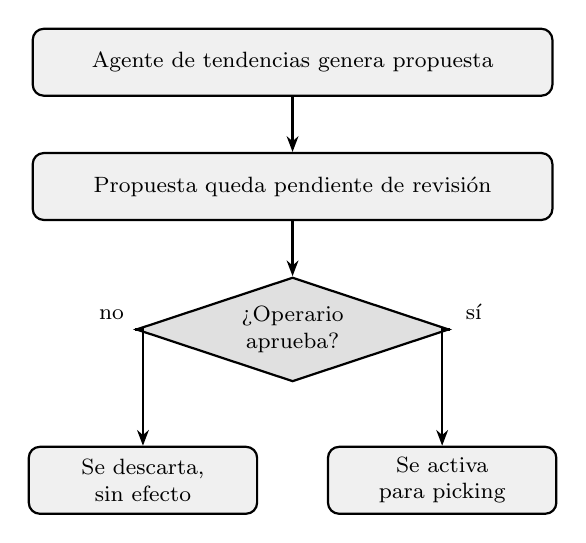
\begin{tikzpicture}[
  font=\footnotesize,
  node distance=7mm and 0mm,
  box/.style={rectangle, draw, rounded corners, minimum width=6.6cm,
    minimum height=0.85cm, align=center, thick, fill=black!6},
  dec/.style={diamond, draw, aspect=3, minimum width=2.6cm,
    minimum height=0.9cm, align=center, thick, fill=black!12},
  arr/.style={-{Stealth[length=2mm]}, thick}
]
\node[box] (a) {Agente de tendencias genera propuesta};
\node[box, below=of a] (b) {Propuesta queda pendiente de revisión};
\node[dec, below=of b] (c) {¿Operario\\ aprueba?};
\node[box, below=8mm of c, xshift=-1.9cm, minimum width=2.9cm] (d) {Se descarta,\\ sin efecto};
\node[box, below=8mm of c, xshift=1.9cm, minimum width=2.9cm] (e) {Se activa\\ para picking};
\draw[arr] (a) -- (b);
\draw[arr] (b) -- (c);
\draw[arr] (c) -| node[above, xshift=-4mm]{no} (d);
\draw[arr] (c) -| node[above, xshift=4mm]{sí} (e);
\end{tikzpicture}
\caption{Flujo de aprobación humano-en-el-bucle para tendencias detectadas
automáticamente.}
\label{fig:approval}
\end{figure}

\subsubsection{Emparejamiento semántico prenda-tendencia}

Una vez aprobada, la descripción de tendencia y la fotografía de cada
referencia de catálogo se proyectan en el mismo espacio de representación
compartido introducido en la Sección~\ref{sec:relwork}-C, lo que permite
calcular una afinidad semántica continua entre ambas mediante similitud
coseno:

\begin{equation}
s_{\text{sem}}(k, t) = \frac{v_{k} \cdot v_{t}}{\lVert v_{k} \rVert \, \lVert v_{t} \rVert} \, \in \, [-1, 1]
\label{eq:sem}
\end{equation}

\noindent donde $v_k$ es la representación visual de la referencia de
catálogo $k$ y $v_t$ es la representación textual de la tendencia $t$. Esta
señal semántica continua se complementa con una señal categórica que
favorece, sin descartar el resto, a las referencias cuya familia de estilo
coincide explícitamente con la detectada por el agente de tendencias:

\begin{equation}
s(k, t) = s_{\text{sem}}(k, t) + \beta \cdot \mathbb{1}\!\left[\,\text{estilo}(k) \in \text{estilo}(t)\,\right]
\label{eq:score}
\end{equation}

\noindent con $\beta$ un peso experimental pequeño frente al rango habitual
de la similitud semántica. Cuando existen varias tendencias activas de forma
simultánea --- distintos mercados o distintos segmentos ---, el score final
de una referencia de catálogo se obtiene agregando la contribución de cada
tendencia relevante, ponderada por su intensidad estimada, de modo que las
tendencias más fuertes dominan el resultado sin anular por completo la
contribución de señales más débiles pero coherentes entre sí.


\subsection{Modo 5: optimización multiobjetivo}

El Modo~5 combina los Modos~3 y 4 dentro de un único criterio de decisión:
la demanda geográfica actúa como restricción dura sobre el conjunto de
referencias elegibles, mientras que la afinidad con tendencias, calculada
mediante la Ecuación~\eqref{eq:score}, actúa como criterio de ordenación
blando dentro de ese conjunto ya filtrado. El sistema calcula un score unificado ponderando la urgencia de reposición geográfica del ERP (peso A) con la similitud semántica de tendencia de CLIP (peso B). El robot prioriza el picking de la caja cuyo score combinado sea mayor, de este modo, un mismo pedido para
un mercado concreto no se resuelve simplemente por disponibilidad de
inventario, sino priorizando, dentro de lo permitido para ese mercado, las
referencias más alineadas con la tendencia vigente. Este modo constituye la
validación final, de extremo a extremo, de la hipótesis central del
trabajo: el cierre completo del bucle entre inteligencia de negocio y
ejecución física.


\subsection{Casos de Uso Ilustrativos y Aportación Esperada}
\label{sec:usecases}

Con el fin de trasladar la arquitectura propuesta a un plano concreto y de
valorar su aportación diferencial frente a la operativa actual de un centro
de distribución de moda, se describen a continuación tres escenarios
ilustrativos. Se trata de ejemplos hipotéticos, construidos para razonar
sobre la aportación esperada del sistema propuesto, y no de resultados
obtenidos sobre una implementación real.

\subsubsection{Escenario 1: reposición por demanda regional}

Considérese un centro de distribución europeo que recibe, de forma
simultánea, un pedido de reposición de 200 unidades para el mercado del
Reino Unido y otro de 150 unidades para el mercado francés, sin más
especificación que el mercado de destino y la cantidad. En la operativa
manual habitual, un operario debe conocer, o consultar, qué referencias del
catálogo están autorizadas para cada mercado antes de iniciar la selección
física, lo que introduce un tiempo de preparación y un riesgo de error
humano crecientes con el tamaño del catálogo. Bajo el Modo~3 propuesto, el
sistema filtra automáticamente el catálogo disponible por mercado de destino
en el instante en que se recibe el pedido, y entrega al planificador de
picking dos listas ya acotadas y priorizadas por disponibilidad de stock,
reduciendo el tiempo de preparación de la orden de trabajo a una fracción del
tiempo actual y eliminando por completo el riesgo de selección de una
referencia no autorizada para su mercado.

\subsubsection{Escenario 2: picking orientado a tendencias virales}

Considérese ahora un escenario en el que el agente de tendencias detecta,
a partir de contenido reciente en redes sociales, una estética de
minimalismo urbano en tonos pastel ganando fuerza en el mercado británico, y
el operario de planta aprueba dicha tendencia desde el panel de operador.
Bajo la operativa actual, esta información --- generada por el departamento
de marketing o por un servicio externo de análisis de tendencias --- rara
vez alcanza a la planta de picking en un plazo útil, y cuando lo hace, su
traducción a una selección concreta de referencias de catálogo depende del
criterio manual de un responsable de producto. Bajo el Modo~4 propuesto, la
tendencia aprobada se traduce automáticamente, en menos de un minuto, en un
reordenamiento de las referencias candidatas dentro del segmento de producto
afectado, de modo que las siguientes órdenes de picking para ese mercado
priorizan, de forma automática, las prendas visualmente más afines a la
estética detectada --- sin que ningún operario de planta necesite tener
conocimiento de moda para tomar esa decisión.

\subsubsection{Escenario 3: gestión integral multiobjetivo}

Combínense ambos escenarios anteriores bajo el Modo~5: un pedido de
reposición para el mercado británico se resuelve seleccionando, dentro del
conjunto de referencias autorizadas para ese mercado, aquellas más afines a
la tendencia de minimalismo urbano vigente. Frente a una operativa actual en
la que estas dos fuentes de información --- demanda geográfica y tendencia
de mercado --- se gestionan, cuando se gestionan, de forma manual y
desacoplada, este escenario ilustra la aportación central del trabajo: un
único sistema robótico capaz de razonar simultáneamente sobre restricciones
de negocio estructuradas y sobre señales de mercado no estructuradas, sin
intervención humana más allá de la aprobación inicial de la tendencia.

\subsubsection{Aportación diferencial frente al estado del arte}

Los tres escenarios anteriores permiten sintetizar la aportación esperada de
este trabajo frente a la revisión de la Sección~\ref{sec:relwork}. Frente a
la literatura de manipulación robótica de textiles, centrada en el reto
físico del agarre, este trabajo añade una capa de decisión de negocio que
determina qué agarrar y en qué orden. Frente a la literatura de
clasificación de prendas por visión, orientada a fotografía de catálogo,
este trabajo aporta una taxonomía y un conjunto de datos propios adaptados a
la condición industrial real de picking. Y frente a la práctica actual de
predicción de tendencias de moda, desacoplada de la operación física, este
trabajo propone un mecanismo concreto --- el emparejamiento semántico de la
Sección~\ref{sec:trends} --- para trasladar esa inteligencia hasta la
decisión robótica, cerrando un bucle IT-OT que, hasta donde alcanza esta
revisión, no se encuentra descrito en la literatura de forma integrada.


\section{Diseño Experimental y Metodología de Validación}
\label{sec:metrics}

Dado que este trabajo se sitúa en su fase de revisión y propuesta, previa a
la implementación, se define a continuación la metodología para validar la
hipótesis planteada. El sistema se someterá a iteraciones de \emph{picking}
con restricciones de aceleración cinemática, registrando tanto los tiempos de ciclo
como la robustez del agarre sobre la caja rígida frente a inercias. La Tabla~\ref{tab:metrics} recoge los objetivos de diseño
previstos para cada componente del sistema, que constituirán el marco de
evaluación del futuro Trabajo Fin de Máster. Se distingue, en particular, un
conjunto de métricas de calidad de percepción y correspondencia, de
métricas de calidad del emparejamiento con tendencias --- de naturaleza más
cualitativa, al no existir un patrón de referencia objetivo para lo que
constituye una selección ``correcta'' frente a una tendencia --- y de
métricas de desempeño físico del picking.

\begin{table*}[!t]
\caption{\textsc{Objetivos de diseño previstos por componente del sistema}}
\label{tab:metrics}
\centering
\footnotesize
\begin{tabular}{@{}llp{7.5cm}c@{}}
\toprule
\textbf{Componente} & \textbf{Métrica} & \textbf{Descripción} & \textbf{Objetivo} \\
\midrule
Clasificación visual & mAP@0.5 & Precisión media sobre los 36 tipos genéricos de la taxonomía & $> 0.85$ \\
Correspondencia de catálogo & Recall@1 & La referencia correcta es la primera candidata & $> 0.60$ \\
Correspondencia de catálogo & Recall@5 & La referencia correcta figura entre las cinco primeras & $> 0.85$ \\
Emparejamiento de tendencias & Precisión@K & Proporción de candidatos alineados con la tendencia entre los K seleccionados & $> 0.70$ \\
Emparejamiento de tendencias & NDCG@K & Calidad del orden de los K candidatos seleccionados & $> 0.75$ \\
Picking robótico & Tasa de éxito de agarre & Proporción de intentos sin fallo mecánico & $> 0.90$ \\
Picking robótico & Tiempo de ciclo & Tiempo entre detección y depósito de la caja & $< 8$ s/caja \\
Sistema (Modo 4) & Latencia extremo a extremo (picking) & Del pedido al inicio de movimiento del robot & $< 2$ s \\
Sistema (Modo 4) & Latencia extremo a extremo (tendencias) & De la ejecución del agente al vector de tendencia activo & $< 60$ s \\
\bottomrule
\end{tabular}
\end{table*}

\section{Plan de Trabajo}
\label{sec:plan}

La Tabla~\ref{tab:plan} resume la planificación prevista para el desarrollo
del Trabajo Fin de Máster que dará continuidad a este trabajo de
investigación tutelado, organizada en fases que respetan las dependencias
técnicas entre modos de operación descritas en la
Sección~\ref{sec:arch}-B: la infraestructura de middleware y control es
condición previa para el Modo~1, que a su vez condiciona el Modo~2 y, a
través de él, la correspondencia de catálogo de la que dependen tanto el
Modo~3 como el Modo~4; el Modo~5 se aborda en último lugar por ser la
composición de los dos anteriores.

\begin{table*}[!t]
\caption{\textsc{Plan de trabajo previsto}}
\label{tab:plan}
\centering
\footnotesize
\begin{tabular}{@{}lp{3.6cm}p{9.5cm}@{}}
\toprule
\textbf{Fase} & \textbf{Periodo} & \textbf{Objetivos clave} \\
\midrule
Teórica & Verano previo al curso & Revisión del estado del arte, definición de arquitectura y de la taxonomía de prendas (este documento) \\
Infraestructura y Modo~1 & Primer trimestre del curso & Puesta en marcha del middleware y del control de robot; detección y singulación de cajas \\
Modo~2 y catálogo & Segundo trimestre & Clasificación por tipo genérico; herramienta de alta de catálogo; correspondencia de referencia exacta \\
Modos 3 y 4 & Tercer trimestre & Reposición geográfica; agente de tendencias; emparejamiento semántico prenda-tendencia \\
Modo 5 y validación & Cuarto trimestre & Optimización multiobjetivo; servoing visual; evaluación de extremo a extremo frente a los objetivos de la Tabla~\ref{tab:metrics} \\
Redacción final & Cierre del curso & Memoria final del Trabajo Fin de Máster y preparación de la defensa \\
\bottomrule
\end{tabular}
\end{table*}

Entre los riesgos identificados para esta planificación destacan la
posibilidad de que la correspondencia de catálogo no alcance de forma
directa los objetivos de precisión fijados en la Tabla~\ref{tab:metrics},
para lo cual se contempla como mitigación un ajuste adicional del espacio de
representación compartido; y la posibilidad de que el tiempo disponible no
sea suficiente para completar el Modo~5 en su forma más ambiciosa, en cuyo
caso se priorizará la validación sólida de los Modos~1 a~4 frente a la
extensión de la optimización conjunta.

\section{Limitaciones y Trabajo Futuro}
\label{sec:future}

Esta propuesta presenta, de forma consciente, tres límites que se documentan
aquí con honestidad, por tratarse de un trabajo de alcance de máster y no de
un sistema de producción.

En primer lugar, el sistema asume un entorno de plegado estandarizado (restricción de contorno) para acotar la complejidad visual de los pliegues. En el entorno real de logística inversa (\emph{fast fashion}), la ropa suele devolverse doblada de formas muy variadas o caóticas; por ello, esta restricción asume una etapa de preprocesamiento (manual o automatizada aguas arriba) donde las prendas se depositan de forma semi-estructurada en las cajas rígidas antes de entrar en la célula bimanual. Así, el sistema resuelve la parte compleja de la correspondencia semántica (Kitting), asumiendo que la singulación inicial caótica se resolvió previamente. En la identificación de referencias se asume un ``overfitting forzado'' con aumentación de datos sobre unas cinco fotografías base. Esta suposición permite centrar la carga de investigación en el emparejamiento semántico multimodal \cite{guo2019imaterialist, radford2021clip}.


En segundo lugar, el filtro categórico del emparejamiento semántico depende
de que el agente de tendencias devuelva siempre un valor perteneciente al
vocabulario cerrado de familias de estilo del catálogo; un modelo de
lenguaje de menor capacidad podría, en ocasiones, devolver un valor fuera de
ese vocabulario, degradando silenciosamente el emparejamiento a su
componente puramente semántico. Se contempla como mitigación una validación
explícita de la salida del modelo frente al vocabulario cerrado antes de
aceptar cualquier tendencia.

En tercer lugar, el etiquetado de estilo de cada referencia de catálogo lo
realiza una persona de forma manual, lo que introduce un riesgo real de
deriva de criterio a medida que crece el número de referencias etiquetadas.
Como trabajo futuro se plantea explorar un etiquetado asistido por modelos
de lenguaje, en el que el sistema proponga automáticamente los atributos de
estilo de una referencia nueva y una persona se limite a confirmarlos o
corregirlos, quedando este planteamiento fuera del alcance del presente
trabajo por no constituir su núcleo de aportación investigadora.

En cuarto lugar, el equilibrio del catálogo entre familias de estilo es, por
construcción, prácticamente estático, mientras que la tendencia detectada es
dinámica; un catálogo desequilibrado hacia unas pocas familias de estilo
dejará a las tendencias detectadas en familias infrarrepresentadas con pocos
candidatos reales entre los que elegir. Se acepta esta limitación para el
alcance de este trabajo, y se señala como línea de trabajo futuro una
estrategia activa de reposición de catálogo por familia de estilo en un
escenario de despliegue de producción real.

\section{Conclusiones}
\label{sec:conclusion}

Este artículo ha revisado el estado del arte en tres campos --- manipulación
robótica de textiles, clasificación de prendas mediante visión por
computador y modelos multimodales visión-lenguaje, y predicción de
tendencias de moda mediante inteligencia artificial --- y ha identificado un
vacío de integración entre ellos: ningún trabajo revisado cierra, de
extremo a extremo, el bucle entre la inteligencia de tendencias generada en
los departamentos de marketing y la ejecución física del picking en un
almacén de moda. A partir de este vacío, se ha propuesto una arquitectura de
sistema robótico bimanual organizada en tres capas y cinco modos de
operación progresivos, sustentada en una taxonomía de prendas diseñada
específicamente para la condición industrial de picking y en un espacio de
representación semántica compartido entre imagen y lenguaje que permite
traducir descripciones textuales de tendencia en decisiones de selección
física de producto. Los escenarios ilustrativos presentados sugieren que
esta integración puede reducir de forma significativa el tiempo de
preparación de pedidos orientados a mercado y habilitar, por primera vez, un
picking robótico sensible a la tendencia de moda vigente sin intervención
manual más allá de la aprobación de negocio. La validación experimental de
esta propuesta, siguiendo el plan de trabajo y los objetivos de diseño
descritos en las Secciones~\ref{sec:plan} y~\ref{sec:metrics}, constituye el
objeto del Trabajo Fin de Máster que da continuidad a esta investigación.

\section*{Contexto del Estudio}
Este documento constituye la fase de revisión del estado del arte y propuesta arquitectónica previa al desarrollo del Trabajo Fin de Máster en la Universidad Carlos III de Madrid.

\begin{thebibliography}{00}

\bibitem{sanchez2018deformable}
J.~Sanchez, J.~A.~Corrales, B.~C.~Bouzgarrou, and Y.~Mezouar, ``Robotic manipulation and sensing of deformable objects in domestic and industrial applications: a survey,'' \emph{The International Journal of Robotics Research}, vol.~37, no.~7, pp.~688--716, 2018.

\bibitem{lui2023textilesurvey}
K.~Lui, W.~W.~Lee, and K.~L.~Lam, ``A Survey on Textile Manipulation for Robotic Systems,'' \emph{IEEE Transactions on Automation Science and Engineering}, vol.~20, no.~4, pp.~3201--3215, 2023.

\bibitem{liu2016deepfashion}
Z.~Liu, P.~Luo, S.~Qiu, X.~Wang, and X.~Tang, ``DeepFashion: Powering
robust clothes recognition and retrieval with rich annotations,'' in
\emph{Proc. IEEE Conf. Computer Vision and Pattern Recognition (CVPR)},
2016, pp.\ 1096--1104.

\bibitem{ge2019deepfashion2}
Y.~Ge, R.~Zhang, L.~Wu, X.~Wang, X.~Tang, and P.~Luo, ``DeepFashion2: A
versatile benchmark for detection, pose estimation, segmentation and
re-identification of clothing images,'' in \emph{Proc. IEEE Conf. Computer
Vision and Pattern Recognition (CVPR)}, 2019, pp.\ 5337--5345.

\bibitem{guo2019imaterialist}
S.~Guo \emph{et~al.}, ``The iMaterialist fashion attribute dataset,'' in
\emph{Proc. IEEE/CVF Int. Conf. Computer Vision Workshops (ICCVW)}, 2019.

\bibitem{jia2020fashionpedia}
M.~Jia, M.~Shi, M.~Sirotenko, Y.~Cui, C.~Cardie, B.~Hariharan, H.~Adam, and
S.~Belongie, ``Fashionpedia: Ontology, segmentation, and an attribute
localization dataset,'' in \emph{Proc. European Conf. Computer Vision
(ECCV)}, 2020, pp.\ 316--332.

\bibitem{xiao2017fashionmnist}
H.~Xiao, K.~Rasul, and R.~Vollgraf, ``Fashion-MNIST: A novel image dataset
for benchmarking machine learning algorithms,'' \emph{arXiv preprint
arXiv:1708.07747}, 2017.

\bibitem{radford2021clip}
A.~Radford \emph{et~al.}, ``Learning transferable visual models from
natural language supervision,'' in \emph{Proc. Int. Conf. Machine Learning
(ICML)}, 2021, pp.\ 8748--8763.

\bibitem{jia2021align}
C.~Jia \emph{et~al.}, ``Scaling up visual and vision-language
representation learning with noisy text supervision,'' in \emph{Proc. Int.
Conf. Machine Learning (ICML)}, 2021, pp.\ 4904--4916.

\bibitem{chia2022fashionclip}
P.~J.~Chia \emph{et~al.}, ``Contrastive language and vision learning of
general fashion concepts,'' \emph{Scientific Reports}, vol.~12, no.~1,
p.~18958, 2022.

\bibitem{liu2023groundingdino}
S.~Liu \emph{et~al.}, ``Grounding DINO: Marrying DINO with grounded
pre-training for open-set object detection,'' \emph{arXiv preprint
arXiv:2303.05499}, 2023.

\bibitem{macenski2022ros2}
S.~Macenski, T.~Foote, B.~Gerkey, C.~Lalancette, and W.~Woodall, ``Robot
Operating System 2: Design, architecture, and uses in the wild,''
\emph{Science Robotics}, vol.~7, no.~66, 2022.

\bibitem{ref17}
Referencia 17 del estado del arte (Llama-3 y cinemática en Edge Computing),
pendiente de integrar en bibliografía final.

\end{thebibliography}

\end{document}
